\documentclass{book}
% Diseño general de página
\usepackage[paperwidth=155mm,
paperheight=230mm,
textwidth=110mm,
textheight=540pt,
centering,
includehead,
includefoot,
headsep=13.5pt,
top=35pt,
footskip=0mm,
footnotesep=13.5pt plus 0.1pt minus 0.1pt]{geometry}

% Idiomas y babel
\usepackage[french,portuguese,italian,english,german,spanish,es-ucroman,es-noshorthands]{babel}
\usepackage[autostyle=true]{csquotes}
\renewcommand{\spanishcontentsname}{Sumario}
\renewcommand{\spanishindexname}{Índice alfabético}

\tracinglostchars=2
\usepackage{fontspec}
\usepackage{microtype}
\newfontfeature{Microtypography}{protrusion=default;expansion=default}
\directlua{fonts.protrusions.setups.default.factor=.5}
\renewcommand{\normalsize}{\fontsize{10pt}{13.5pt}\selectfont}
\topskip=13.5pt

% tipografía Libertinus
\setmainfont{Libertinus Serif}
[Numbers={OldStyle,Proportional},Ligatures=TeX,Scale=1.18]

% diseño tipográfico con Minion Pro 3
% \setmainfont{Minion 3}
% [Numbers={OldStyle,Proportional},Ligatures=TeX,Scale=1.2]

\setsansfont[Scale=MatchLowercase,
Ligatures=TeX,
Extension=.otf,
UprightFont=*-Regular,
ItalicFont=*-Italic,
BoldFont=*-SemiBold,
BoldItalicFont=*-SemiBoldItalic]{IBMPlexSansCondensed}

\setmonofont[Scale=0.91,
Extension=.otf,
UprightFont=*-Regular,
ItalicFont = IBMPlexMono-Italic.otf,
BoldFont = IBMPlexMono-Bold.otf,
BoldItalicFont = IBMPlexMono-BoldItalic.otf]{IBMPlexMono.otf}

% configuración de los valores decimales de los cuadros
\usepackage{siunitx}
\sisetup{output-decimal-marker={.},
         group-separator={\,},
         group-minimum-digits=3,
         table-text-alignment=center,
         detect-all}

% para comentarios y alertas
\usepackage{easyReview}

% control de ruptura de linea
\usepackage{linebreaker}
\linebreakersetup{
	maxtolerance=90,
	maxemergencystretch=1em,
	maxcycles=4
}

% paquetes varios
\usepackage{froufrou}
\usepackage{nccfoots}
\usepackage{booktabs}
\usepackage{rotating}
\usepackage{graphicx}
\usepackage{svg}
\usepackage[final]{pdfpages}
\usepackage[labelfont=bf,font=small,labelsep=period,format=plain]{caption}
\usepackage{ragged2e}
\usepackage{xcolor}

% diseño de listas
\usepackage{enumitem}
\setlist{nosep,topsep=-\parskip}

% rediseño del epígrafe
\newcommand{\epigraph}[2]{%
	\par\nobreak\noindent\par\nobreak\vspace{.5\baselineskip}
	\hfill{\small\begin{tabular}{@{}>{\raggedright\arraybackslash}m{.65\textwidth}@{}}
			#1 \\[1ex]
			\midrule
			#2
	\end{tabular}}
	\vspace{.5\baselineskip}
}

% niveles para los contadores
\setcounter{tocdepth}{1}
\setcounter{secnumdepth}{4}

% dibujo de caja contenedora, solo para desarrollo
%\usepackage{showframe}
%\renewcommand\ShowFrameLinethickness{0.1pt}
%\renewcommand\ShowFrameColor{\color{blue}}

% cruces de corte
%\usepackage[width=18truecm,height=25.5truecm,cam,center]{crop}
%\newcommand*\infofont[1]{\sf{\footnotesize #1 (alberto.alejandro.moyano@gmail.com)}}
%\crop[font=infofont]

%% fondo gris para no arruinarme la vista
%\pagecolor{lightgray!40}

% diseño del pie de página
\usepackage[bottom,stable,hang]{footmisc}
\makeatletter
\patchcmd{\@footnotetext}{\footnotesize}{\small}{}{}% tamaño del cuerpo del texto del footnote
\makeatother
\renewcommand*{\thefootnote}{\scriptsize\sf{[\arabic{footnote}]}}% tamaño del cuerpo de puntero del footnote

% KOMA script
\usepackage{scrextend}
% \KOMAoptions{footnotes=multiple}% maybe you want to use this option?
\newcommand*\footnotemarkspace{0em} % set distance of the footnote text from the margin
\deffootnote{\footnotemarkspace}% use distance from above
{\parindent}% paragraph indent in footnotes (footnotes should never have paragraphs!)
{\makebox[\footnotemarkspace][r]{\llap{\thefootnotemark\quad}}} % footfont with period for footnote marks in footnote
%   {\makebox[\footnotemarkspace][l]{\footfont\phantom{99}\llap{\thefootnotemark.}}} % footfont with period for footnote marks in footnote

% cambiar la font specification for the name "PART"
\renewcommand\thepart{\arabic{part}}

% AJUSTE PARA UTILIZAR SUBTITULOS, CHAPTER CON ce MAYÚSCULA \Chapter{}{}
% \usepackage{relsize} %Package to set relative font size (\smaller, \larger)
\newcommand\Chapter[2]{
	\chapter[#1]{#1\\ {\fontsize{12pt}{14.4pt}\selectfont#2}}
}

\usepackage{titletoc}
% partes
\titlecontents{part}[0em]
{\addvspace{5pt}\sf\bfseries\normalsize\selectfont\filright}
{\contentslabel[\thecontentslabel]{2.5pc}}{}{}

% capitulo
\titlecontents{chapter}[2pc]
{\addvspace{.4em}\sf\selectfont\filright}
{\contentslabel{2pc}}
{\hspace*{-2pc}}%
{\titlerule*[1pc]{.}\contentspage[\hspace*{-3pc} {\rm\small\thecontentspage}]}%
[]

\titlecontents{section}[4.5pc]
{\small\filright}
{\contentslabel{2.5pc}}
{\hspace*{-2.5pc}}
{\titlerule*[1pc]{.}\contentspage}

% %% diseño de sección
% \titlecontents*{section}[2.5pc]
% {\small\selectfont\filright}
% {{\sffamily{\thecontentslabel}} \ }{}
% { [\textbf{\thecontentspage}]}[][\ \textbullet\ ][]

% \titlecontents*{section}[2.5pc]
% {\footnotesize\selectfont\raggedright}
% {\textbf{\thecontentslabel\adddot}\addspace}
% % {\thecontentslabel.\addspace}% despues de terminar con Tucumán usar este
% {}
% {~[\thecontentspage].\addspace}[]
% % {\addspace[\thecontentspage].\addspace}[]

% CORRIJE LA POSICIÓN DE LOS NUMEROS EN EL ÍNDICE DE FIGURAS Y CUADROS
\makeatletter
\renewcommand{\l@figure}{\@dottedtocline {1}{0}{2.5pc}}
\renewcommand{\l@table}{\@dottedtocline {1}{0}{2.5pc}}
\makeatother

\usepackage[sf,bf,compact,topmarks,calcwidth,pagestyles,clearempty,newlinetospace]{titlesec}
%diseño de parte
\makeatletter
\def\@part[#1]#2{\ifnum \c@secnumdepth >-2\relax
	\refstepcounter{part}%

	\addcontentsline{toc}{part}{Parte \thepart
		\hspace{1em}#1}\else

	\addcontentsline{toc}{part}{#1}\fi
	\markboth{}{}%
	{\centering
		\interlinepenalty \@M
		\ifnum \c@secnumdepth >-2\relax
		\sf\LARGE\selectfont \partname~\thepart
		\par
		\vskip 20\p@\fi
		\sf\LARGE\selectfont
		#2\par}\@endpart}
\makeatother

%diseño de capitulo
\titleformat{\chapter}[display]
% {\sf \LARGE}
% {\filleft {\chaptertitlename} \thechapter}
% {2ex}{\filright}[]
{\Large}
{\vspace{-2.5cm}\centering{\textsc{\MakeLowercase\chaptertitlename}}~\thechapter}
{1.5cm}
{\filright\sf\LARGE}
[]
% \titlespacing{\chapter}{0pt}{-9ex}{0pt}

%diseño de seccion
\titleformat{\section}[hang]
{\sf\bfseries\large\raggedright}
{\thesection}{.5em}{}[]
\titlespacing{\section}
{\parindent}{18pt plus .1pt minus -.1pt}{6.75pt}

%diseño de subseccion
\titleformat{\subsection}[hang]
{\sf\large\raggedright}
{\thesubsection}{.5em}{}[]
\titlespacing{\subsection}
{\parindent}{18pt plus .1pt minus -.1pt}{6.75pt}

%diseño de subsubseccion
\titleformat{\subsubsection}[hang]
{\rm\bfseries\normalsize\raggedright}
{\thesubsubsection}{.5em}{}[]
\titlespacing{\subsubsection}
{\parindent}{18pt plus .1pt minus -.1pt}{6.75pt}

%diseño de parrafo para usar con los autores de compilaciones
\titleformat{\paragraph}[runin]
  {\normalfont\sc\MakeLowercase}
  {}{0em}{}
  [\mbox{ --- }]
\titlespacing{\paragraph}
  {0pt}% antes de la raya
  {6.75pt plus .1pt minus -.1pt}% antes del párrafo
  {0pt}% después de la raya

%diseño de subparrafo TRUCO PARA CENTRAR NUMEROS DE NIGRA
\titleformat{\subparagraph}[hang]
{\sf\bfseries\large\centering}
{\thesubparagraph}{.5em}{}[]
\titlespacing{\subparagraph}
{\parindent}{1pc plus .1pc minus -.2pc}{.5pc}

% DISEÑO DE CABEZALES
\renewpagestyle{plain}[]{% \footrule
\setfoot{}{}{}}
\newpagestyle{myps}[]{%
\setfoot[][][]{}{}{}
\sethead[\sf \textbf{\usepage}][][\sf \TheAuthor]
{\sf \chaptertitle}{}{\sf \textbf{\usepage}}
}
\pagestyle{myps}

\newcommand{\TheAuthor}{}
\newcommand{\Author}[1]{\renewcommand{\TheAuthor}{#1}}

% Ajustes de viudas y huérfanas
\raggedbottom
\clubpenalty=10000
\widowpenalty=10000
% \hyphenpenalty=3000
\finalhyphendemerits% evitamos el corte en la última línea del párrafo
%% CON ESTAS 2 INSTRUCCIONES NUNCA VA A GUIONIZAR PALABRAS MENORES A 7 CARACTERES
% \lefthyphenmin3 %% determina el minimo de caracteres de final de linea a la izquierda
% \righthyphenmin3 %% determina el minimo de caracteres de final de linea a la derecha

% NUEVO TIPO DE ENTORNO FLOTANTE PARA FOTOGRAFIAS (\listofimagen)
\usepackage{newfloat}
\DeclareFloatingEnvironment[
fileext=lop,
listname={Índice de imágenes},
name=Imagen,
placement=ht,
%within=section,% activate it if you want
%chapterlistsgaps=on,% meaningful only if chapters exist
]{imagen}

% DISEÑO DE RAYA DEL MEDIO
\makeatletter
\def\thinskip{\hskip 0.16667em\relax}
\def\endash{--}
\def\emdash{\endash-}
\def\d@sh#1#2{\unskip#1\thinskip#2\thinskip\ignorespaces}
\def\dash{\d@sh\nobreak\endash}
\def\Dash{\d@sh\nobreak\emdash}
\def\ldash{\d@sh\empty{\hbox{\endash}\nobreak}}
\def\rdash{\d@sh\nobreak\endash}
\def\Ldash{\d@sh\empty{\hbox{\emdash}\nobreak}}
\def\Rdash{\d@sh\nobreak\emdash}
\def\hyph{-\penalty\z@\hskip\z@skip}
\def\slash{/\penalty\z@\hskip\z@skip}
\makeatother

% CENTRADO DEL AUTOR DE LOS CAPITULOS
\newcommand\nombreautor[1]{\textsc{\MakeLowercase{#1}}}

% CITA CON CAMBIO DE TAMAÑO TIPOGRAFICO
\renewenvironment{quote}
  {\normalsize\list{}{\sf\leftmargin=14pt \rightmargin=0pt}%
   \item\relax}
  {\endlist}

% CONFIGURACIÓN PARA BIBLATEX
\usepackage[style=philosophy-modern,
sortcites=true,
lowscauthors=true,
scauthorsbib=true,
annotation=true,
backend=bibtex8,
labeldateparts=true,
backref=true,
useprefix=true,
citereset=chapter,
indexing=cite,
relatedformat=brackets,
publocformat=loccolonpub,
volnumformat=strings,
latinemph=true,
inbeforejournal=true,
shorthandintro=true,
texencoding=utf8,
bibencoding=utf8,
uniquelist=minyear]{biblatex}

%GENERAR LOS INDICES, DESACTIVAMOS LAS OPCIONES PARA TITULOS
\renewbibmacro*{bibindex}{%
  \ifbibindex
    {\indexnames{author}%
     \indexnames{editor}%
     \indexnames{translator}%
     \indexnames{commentator}}
    {}}

\renewbibmacro*{citeindex}{%
  \ifciteindex
    {\indexnames{author}%
     \indexnames{editor}%
     \indexnames{translator}%
     \indexnames{commentator}}
    {}}

% CAMBIAMOS URL PARA QUE APAREZCA LA LEYENDA EN LINEA
\makeatletter
\newrobustcmd{\mkbiblege}[1]{%
	\begingroup
	\blx@blxinit
	\blx@setsfcodes
	<#1>
	\endgroup}
\makeatother

\DeclareFieldFormat{url}{\bibstring{url}\space\mkbiblege{\url{#1}}}

% REDEFINIR EL FORMATO DE CITADO EN PÁGINA 00
% \DeclareFieldFormat{pagerefformat}{\mkbibparens{{\color{red}\mkbibemph{#1}}}}
\renewbibmacro*{pageref}{%
	\iflistundef{pageref}
	{}
	{\printtext[pagerefformat]{%
			\ifnumgreater{\value{pageref}}{1}
			{\bibstring{backrefpages}\ppspace}
			{\bibstring{backrefpage}\ppspace}%
			\printlist[pageref][-\value{listtotal}]{pageref}}}}

% DECLARO UNA ALIAS PARA TRATAR MOVIE COMO MISC
\DeclareBibliographyAlias{movie}{misc}

% PONE PUNTO Y COMA ENTRE NOMBRE DE VARIOS AUTORES
\renewcommand*{\multinamedelim}{\addsemicolon\space}

% CAMBIA LA TIPOGRAFIA DE LA BIBLIOGRAFIA
\renewcommand*{\annotationfont}{\small\sf}
\renewcommand*{\bibfont}{\small}
\setlength{\bibhang}{3\parindent}%modifico el valor por default (4) de indentacion del año

\defcounter{biburlnumpenalty}{3000}
\defcounter{biburlucpenalty}{6000}
\defcounter{biburllcpenalty}{9000}

%% REDISEÑO PARA OBTENER MODO LARGO EN ALGUNAS ENTRADAS
\NewBibliographyString{organizator}
\NewBibliographyString{organizators}
\NewBibliographyString{byorganizator}
\NewBibliographyString{cordinator}
\NewBibliographyString{cordinators}
\NewBibliographyString{bycordinator}
\NewBibliographyString{direction}
\NewBibliographyString{directions}
\NewBibliographyString{bydirection}
\NewBibliographyString{maestriathesis}
\NewBibliographyString{ingenieriathesis}
\NewBibliographyString{gradothesis}
\NewBibliographyString{licenciaturathesis}
\NewBibliographyString{origpubbare}
\NewBibliographyString{especialthesis}
\NewBibliographyString{documentjob}
\NewBibliographyString{posgradothesis}
\NewBibliographyString{magisterthesis}
\NewBibliographyString{dirigida}% MODIFICACIONES PARA FILMES
\NewBibliographyString{dirigidas}
\NewBibliographyString{bydirigida}
\NewBibliographyString{escrita}
\NewBibliographyString{escritas}
\NewBibliographyString{byescrita}
\NewBibliographyString{elenco}
\NewBibliographyString{elencos}
\NewBibliographyString{byelenco}

\DefineBibliographyStrings{spanish}{%
	dirigida         = {direcci\'on},
	dirigidas        = {direcci\'on},
	bydirigida       = {Direcci\'on de},
	escrita          = {escrita},
	escritas         = {escrita},
	byescrita        = {escrita por},
	elenco           = {act\'uan:},
	elencos          = {act\'uan:},
	byelenco         = {act\'uan:},
	part             = {tomo},
	january          = {enero},
	february         = {febrero},
	march            = {marzo},
	april            = {abril},
	may              = {mayo},
	june             = {junio},
	july             = {julio},
	august           = {agosto},
	september        = {septiembre},
	october          = {octubre},
	november         = {noviembre},
	december         = {diciembre},
	see              = {v\'ease},
	seealso          = {v\'ease tambi\'en},
	backrefpage      = {re\-fe\-ren\-cia ci\-ta\-da en p\'agi\-na},
	backrefpages     = {re\-fe\-ren\-cia ci\-ta\-da en p\'agi\-nas},
	seenote          = {v\'ease nota},
	quotedin         = {citado en},
	idem             = {\'{\i}dem},
	idemsf           = {\'{\i}dem},
	idemsm           = {\'{\i}dem},
	idemsn           = {\'{\i}dem},
	idempf           = {\'{\i}dem},
	idempm           = {\'{\i}dem},
	idempn           = {\'{\i}dem},
	idempp           = {\'{\i}dem},
	ibidem           = {\emph{ibidem}},
	prepublished     = {previamente publicado},
	nodate           = {sin fecha},
	withcommentator  = {con comentario de},
	withannotator    = {con notas de},
	withintroduction = {con introduci\'on de},
	withforeword     = {con pr\'ologo de},
	withafterword    = {con ep\'{\i}logo de},
	bycollaborator   = {con colaboraci\'{o}n de},
	andothers        = {\emph{et al\adddot}},
	organizator      = {org\adddot},
	organizators     = {orgs\adddot},
	byorganizator    = {org\adddot\addspace por},
	cordinator       = {coord\adddot},
	cordinators      = {coords\adddot},
	bycordinator     = {coord\adddot\addspace por},
	direction        = {dir\adddot},
	directions       = {dirs\adddot},
	bydirection      = {dir\adddot\addspace por},
	mathesis         = {Tesis de Maestr\'{\i}a},
	ingenieriathesis = {Tesis de Ingenier\'{\i}a},
	magisterthesis   = {Tesis de Mag\'ister},
	phdthesis        = {Tesis de Doctorado},
	gradothesis      = {Tesis de Grado},
	licenciaturathesis = {Tesis de Licenciatura},
	posgradothesis   = {Tesis de Posgrado},
	especialthesis   = {Tesis de Especializaci\'{o}n},
	documentjob      = {documento de trabajo},
	urlseen          = {visitado el\addspace},
	translationof    = {trad\adddot\addspace de},
	translationas    = {original publicado en},
	url              = {recuperado de},
	origpubbare      = {orig\adddotspace pub\adddotspace},
	newseries        = {nueva \'epoca},
	oldseries        = {antigua \'epoca},
	byeditorfo       = {ed\adddotspace y pr\'ol\adddotspace por},
	byeditorco       = {ed\adddotspace y com\adddotspace por},
	bytranslatorfo   = {traducido \lbx@lfromlang\ y prologado por},
	pagetotal        = {p\'ags},
	pagetotals       = {p\'ags},
	techreport       = {informe t\'ecnico},
	resreport        = {reporte de investigaci\'{o}n},
	file             = {archivo},
	patent           = {patente},
	patentde         = {patente alemana},
	patenteu         = {patente europea},
	patentfr         = {patente francesa},
	patentuk         = {patente brit\'anica},
	patentus         = {patente estadounidense},
	patreq           = {solicitud de patente},
	patreqde         = {solicitud de patente alemana},
	patreqeu         = {solicitud de patente europea},
	patreqfr         = {solicitud de patente francesa},
	patrequk         = {solicitud de patente brit\'anica},
	patrequs         = {solicitud de patente estadounidense},
	bycompiler       = {comp\adddotspace por},
}

% corrección para año original
\makeatletter
\renewbibmacro*{transorigstring}{%
  \iffieldundef{reprinttitle}%
  {\printtext{\ifdefstring{\bbx@origfields}{origed}
      {\bibstring{origpubbare}}%
      {\bibstring{translationas}}}\nopunct}%
  {\printtext{\bibstring{reprint}}}\nopunct}
\makeatother

% generamos los índices % columnsep=20pt,columnseprule
\usepackage[xindy]{imakeidx}
\makeindex
\makeindex[name=names,title={Índice de autoras y autores}]
\makeindex[name=concepto,title={Índice de conceptos}]
\makeindex[name=onomastico,title={Índice onomástico}]

\usepackage{esindex}
\DeclareIndexNameFormat{default}{%
	\usebibmacro{index:name}{\esindex[names]}
	{\namepartfamily}
	{\namepartgiven}
	{\namepartprefix}
	{\namepartsuffix}}
\renewbibmacro*{citeindex}{%
	\ifciteindex
	{\indexnames{labelname}}
	{}}
\usepackage[totoc]{idxlayout}

% generamos los glosarios
\usepackage[acronym,sanitizesort,toc=true,nonumberlist]{glossaries}
\preto\chapter{\glsresetall}
\makenoidxglossaries
\renewcommand{\glsnamefont}[1]{\sf\textbf{\textup{#1}}}

% Diseño y estilo a glosario y acrónimo
\newglossarystyle{crossreflist}%
{% base it on list (adapt as required)
	\renewcommand*{\glossentry}[2]{%
		\item[\glsentryitem{##1}%
		\glstarget{##1}{\glossentryname{##1}}]
		\glossentrydesc{##1}\glspostdescription\space ##2%
		% check if the user1 key has been supplied:
		\ifglshasfield{useri}{##1}%
		{% do cross-reference
			\newline
			\glsletentryfield{\crossrefs}{##1}{useri}%
			\glsseeformat[\emph{Véase:}]{\crossrefs}{}%
		}%
		{}%
	}%
}
\setglossarystyle{crossreflist}

% deshabilitamos mostrar el número de página
%\renewcommand{\glossaryentrynumbers}[1]{Véase página #1.}
\renewcommand{\delimN}{, }
\renewcommand{\delimR}{--}

% Instrucciones de salida
%\printnoidxglossary[type=\acronymtype,title={Índice de siglas}]
%\printnoidxglossary[title={Glosario de términos}]

\usepackage{url}%[allowmove]
\Urlmuskip = 0mu plus 1mu
\def\UrlBreaks{\do\a\do\b\do\c\do\d\do\e\do\f\do\g\do\h\do\i\do\j\do\k\do\l\do\m\do\n\do\o\do\p\do\q\do\r\do\s\do\t\do\u\do\v\do\w\do\x\do\y\do\z\do\A\do\B\do\C\do\D\do\E\do\F\do\G\do\H\do\I\do\J\do\K\do\L\do\M\do\N\do\O\do\P\do\Q\do\R\do\S\do\T\do\U\do\V\do\W\do\X\do\Y\do\Z\do0\do1\do2\do3\do4\do5\do6\do7\do8\do9\do=\do.\do:\do\%\do?\do_\do-\do+\do/\do\#\do~}
\def\UrlFont{\rm}

\usepackage{ifthen}

% fin del preambulo
% se define una variable condicional para cada formato de salida
% a conditional variable is defined for each output format
\newif\ifPDF%
\newif\ifBNPDF%
\newif\ifEPUB%
\newif\ifHTML%
\newif\ifHTMLcinco%
\newif\ifJATS%
\newif\ifODT%

 \PDFtrue
% \BNPDFtrue
% \EPUBtrue
% \HTMLtrue
% \HTMLcincotrue
% \JATStrue
% \ODTtrue

% agregamos las referencias
% we added the references
\addbibresource{./files/gbTeXbib-CHARLAMATE.bib}

% agregamos el glosario
% we added the glossary

\newglossaryentry{@glo194-clai}{
type = \acronymtype,
name         = {CLAI},
description  = {Consejo Latinoamericano de Iglesias},
first        = {Consejo Latinoamericano de Iglesias (CLAI)},
text         = {CLAI},
}
\newglossaryentry{@glo195-coas}{
type = \acronymtype,
name         = {COAS},
description  = {Corriente de Organización y Acción Sindical},
first        = {Corriente de Organización y Acción Sindical (COAS)},
text         = {COAS},
}
\newglossaryentry{@glo200-latex}{
name         = {LaTeX},
description  = {es un sistema de composición de tipografía de alta calidad; incluye características diseñadas para la producción de documentación técnica y científica. LaTeX es la norma de facto para la comunicación y publicación de documentos científicos. Está disponible como software libre},
text         = {LaTeX},
}
\newglossaryentry{@glo201-ceheal}{
type = \acronymtype,
name         = {CEHEAL},
description  = {Centro de Estudios de Historia Económica Latinoamericana y Argentina},
first        = {Centro de Estudios de Historia Económica Latinoamericana y Argentina (CEHEAL)},
text         = {CEHEAL},
}
\newglossaryentry{@glo202-joseingenieros}{
name         = {José Ingenieros},
description  = {(nacido como Giuseppe Ingegnieri,​ Palermo, 24 de abril de 1877 - Buenos Aires, 31 de octubre de 1925) fue un médico, psiquiatra, psicólogo, criminólogo, farmacéutico, sociólogo, filósofo, masón, teósofo, ​escritor y docente ítaloargentino. Su libro \emph{Evolución de las ideas argentinas} marcó rumbos en el entendimiento del desarrollo histórico de Argentina como nación. Se destacó por su influencia entre los estudiantes que protagonizaron la Reforma Universitaria de 1918},
text         = {José Ingenieros},
}

% los metadatos son opcionales en el PDF a diferencia del resto que es obligatorio y se cargan automáticamente
% the metadata is optional in the PDF, unlike the rest which is mandatory and loaded automatically
\ifODT
\usepackage[unicode,hyperindex=true]{hyperref}
\else
	\ifPDF
	% control de inconsistencias de principio y fin de linea
	% inconsistency control of start and end of line (homeoarchy)
	\usepackage[hyphenation,homeoarchy,draft,homeoarchywordcolor=yellow,homeoarchycharcolor=yellow]{impnattypo}
	\usepackage[allcolors=magenta,colorlinks]{hyperref}
	\usepackage{hyperxmp}
	\hypersetup{
pdfauthor={},
pdfdate={0000-00},
pdfcopyright={Copyright},
pdflicenseurl={https://es.wikipedia.org/wiki/Copyright},
pdfpubtype={book},
pdflang={es-ES},
pdfmetalang={es},
pdfrendition={default},
pdfx={pdf/A},
pdftitle={},
pdfcreator={gbTeXpublisher},
pdfproducer={Ecosistema de LaTeX},
unicode=true,
bookmarks=true,
pdfdisplaydoctitle=true,
pdfnewwindow=true
}

	\else
		\ifBNPDF
		\usepackage[cam,width=18truecm,height=25.5truecm,center]{crop}
		\usepackage[hidelinks]{hyperref}
		\usepackage{hyperxmp}
		\hypersetup{
pdfauthor={},
pdfdate={0000-00},
pdfcopyright={Copyright},
pdflicenseurl={https://es.wikipedia.org/wiki/Copyright},
pdfpubtype={book},
pdflang={es-ES},
pdfmetalang={es},
pdfrendition={default},
pdfx={pdf/A},
pdftitle={},
pdfcreator={gbTeXpublisher},
pdfproducer={Ecosistema de LaTeX},
unicode=true,
bookmarks=true,
pdfdisplaydoctitle=true,
pdfnewwindow=true
}

		\else
			\ifEPUB
			\usepackage[hyperindex=true,allcolors=magenta,colorlinks]{hyperref}
			\fi
		\fi
	\fi
\fi

\begin{document}
\frontmatter

\ifEPUB%
	\ifdefined\HCode
	\phantomsection
	\addcontentsline{toc}{section}{Portada}
	\coverimage{./media/cover.png}
	\clearpage
	\fi
\fi

\ifPDF
% página 1
\newpage
\thispagestyle{empty}
{\textcolor{white}{.}}

% página 2
\newpage
\thispagestyle{empty}
{\textcolor{white}{.}}

% página 3
\newpage
\thispagestyle{empty}
{\textcolor{white}{.}}

\vspace{30mm}

\begin{center}
	\LARGE{Mate con editorxs}
\end{center}

% página 4
\newpage
\thispagestyle{empty}
{\textcolor{white}{.}}

% página 5
\newpage
\thispagestyle{empty}
\begin{center}%,draft
{\sc\large{alberto moyano}}\\ %compiladoras
\end{center}

\vspace{30mm}

\begin{center}
\LARGE{Mate con editorxs}\\\vspace{10mm}

\Large{Charlas del CAICYT}
\end{center}

\vfill

\begin{figure}[b]
\centering

\includegraphics[width=40mm]{./media/mate.png}
\end{figure}

% página 6
\newpage
\thispagestyle{empty}
\begin{figure}[t]
\centering
\vspace{-10mm}

\includegraphics[width=30mm]{./media/logo-LaTeX.png}\\
%\sc{colección...}%
\end{figure}

\noindent Alberto Moyano \\
\noindent Mate con editorxs. Charlas del CAICYT. 1a ed. Buenos Aires: 2024.\\
\noindent 000 p.; 15.5x23 cm. ISBN 978-950-000-000-0 \\
\noindent 1. \\
\noindent CDD .\\
\noindent Fecha de catalogación: 00/00/2024 \\
\noindent \textcopyright~2024, Alberto Moyano \\
\noindent \textcopyright~2024, Ediciones Imago Mundi\\
\noindent Imagen de tapa: .\\
\noindent Hecho el depósito que marca la ley 11.723\\
\noindent Impreso en Argentina, tirada de esta edición: 000 ejemplares\\

\vfill

\noindent Ninguna parte de esta publicación, incluido el diseño de cubierta, puede ser reproducida, almacenada o transmitida de manera alguna ni por ningún medio, ya sea eléctrico, químico, mecánico, óptico, de grabación o de fotocopia, sin permiso previo por escrito del editor. Este libro se terminó de imprimir en el mes de xxxx de 2024 en San Carlos Impresiones, Virrey Liniers 2203, Ciudad Autónoma de Buenos Aires, República Argentina.

\else
	\ifBNPDF
	% página 1
\newpage
\thispagestyle{empty}
{\textcolor{white}{.}}

% página 2
\newpage
\thispagestyle{empty}
{\textcolor{white}{.}}

% página 3
\newpage
\thispagestyle{empty}
{\textcolor{white}{.}}

\vspace{30mm}

\begin{center}
	\LARGE{Mate con editorxs}
\end{center}

% página 4
\newpage
\thispagestyle{empty}
{\textcolor{white}{.}}

% página 5
\newpage
\thispagestyle{empty}
\begin{center}%,draft
{\sc\large{alberto moyano}}\\ %compiladoras
\end{center}

\vspace{30mm}

\begin{center}
\LARGE{Mate con editorxs}\\\vspace{10mm}

\Large{Charlas del CAICYT}
\end{center}

\vfill

\begin{figure}[b]
\centering

\includegraphics[width=40mm]{./media/mate.png}
\end{figure}

% página 6
\newpage
\thispagestyle{empty}
\begin{figure}[t]
\centering
\vspace{-10mm}

\includegraphics[width=30mm]{./media/logo-LaTeX.png}\\
%\sc{colección...}%
\end{figure}

\noindent Alberto Moyano \\
\noindent Mate con editorxs. Charlas del CAICYT. 1a ed. Buenos Aires: 2024.\\
\noindent 000 p.; 15.5x23 cm. ISBN 978-950-000-000-0 \\
\noindent 1. \\
\noindent CDD .\\
\noindent Fecha de catalogación: 00/00/2024 \\
\noindent \textcopyright~2024, Alberto Moyano \\
\noindent \textcopyright~2024, Ediciones Imago Mundi\\
\noindent Imagen de tapa: .\\
\noindent Hecho el depósito que marca la ley 11.723\\
\noindent Impreso en Argentina, tirada de esta edición: 000 ejemplares\\

\vfill

\noindent Ninguna parte de esta publicación, incluido el diseño de cubierta, puede ser reproducida, almacenada o transmitida de manera alguna ni por ningún medio, ya sea eléctrico, químico, mecánico, óptico, de grabación o de fotocopia, sin permiso previo por escrito del editor. Este libro se terminó de imprimir en el mes de xxxx de 2024 en San Carlos Impresiones, Virrey Liniers 2203, Ciudad Autónoma de Buenos Aires, República Argentina.

	\fi
\fi

\ifPDF
\Author{Sumario}
\else
	\ifBNPDF
	\Author{Sumario}
	\fi
\fi

\tableofcontents

\chapter{Frontmatter}

La formación de \gls{@glo202-joseingenieros}\index[onomastico]{Ingenieros, José} fue universitaria y a diferencia del lugar tradicional del docente y del académico, su obra adquirió una marcada proyección política logrando complejas derivaciones que no son fácilmente encuadrables en un solo espacio partidario, si bien sus ideas estuvieron ligadas mayoritariamente a la tradición de izquierda socialista. Su vida y su obra habilitaron una diversidad de relecturas, de articulaciones políticas y de reapropiaciones teóricas. Esta particularidad caracterizó a \gls{@glo195-coas} y también a muchos de sus compañeros de militancia como el mexicano José Vasconcelos\index[onomastico]{Vasconcelos, José} o los argentinos Leopoldo Lugones\index[onomastico]{Lugones, Leopoldo} y Manuel Ugarte\index[onomastico]{Ugarte, Manuel} \parencite{@3070-TARKOVSKI1995}.

\mainmatter

\chapter{MainmatterA}

\section{SecciónA}

Esta obra colectiva da continuidad a uno de los programas centrales impulsados por el \gls{@glo201-ceheal} desde su creación en 2019: el estudio de las ideas y del pensamiento económico en su vínculo con la implementación de políticas económicas.\footnote{Una nota a pie de página.}

La secuencia de Fibonacci es una serie matemática en la cual cada número es la suma de los dos anteriores, comenzando generalmente con 0 y 1. La fórmula general para la secuencia de Fibonacci se puede expresar matemáticamente de la siguiente manera:

$$F(n) = F(n-1) + F(n-2)$$

\ifPDF
\froufrou
\else
	\ifBNPDF
	\froufrou
	\else
		\ifODT
		\begin{center} * * * \end{center}
		\fi
	\fi
\fi

\section{SecciónAA}

Esta obra colectiva da continuidad a uno de los programas centrales impulsados por el \gls{@glo201-ceheal} desde su creación en 2019: el estudio de las ideas y del pensamiento económico en su vínculo con la implementación de políticas económicas\index[concepto]{Políticas económicas para la sociedad} \parencite{@940-SHUMWAY1999}.

\chapter{MainmatterB}

\section{SecciónB}

Esta obra colectiva da continuidad a uno de los programas centrales impulsados por el \gls{@glo201-ceheal} desde su creación en 2019: el estudio de las ideas y del pensamiento económico en su vínculo con la implementación de políticas económicas.

\ifPDF%
\begin{figure}[!ht]
\centering
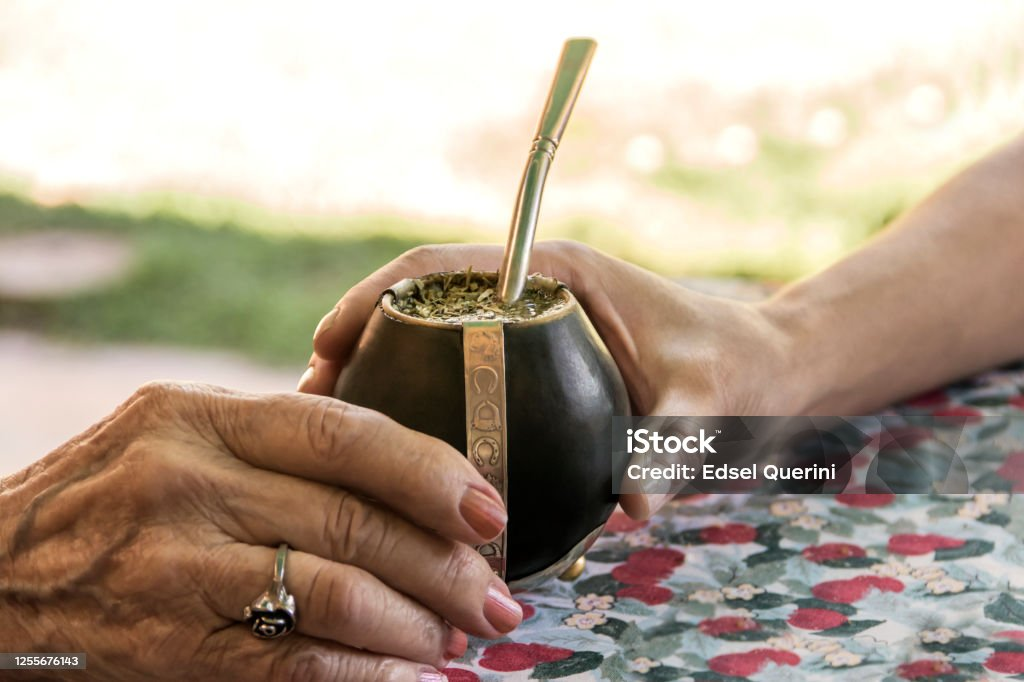
\includegraphics[width=\textwidth]{./media/imagen1.jpg}
\caption{Este es el epígrafe de la figura a color.}
\end{figure}
\else
	\ifBNPDF%
	\begin{figure}[!ht]
	\centering
	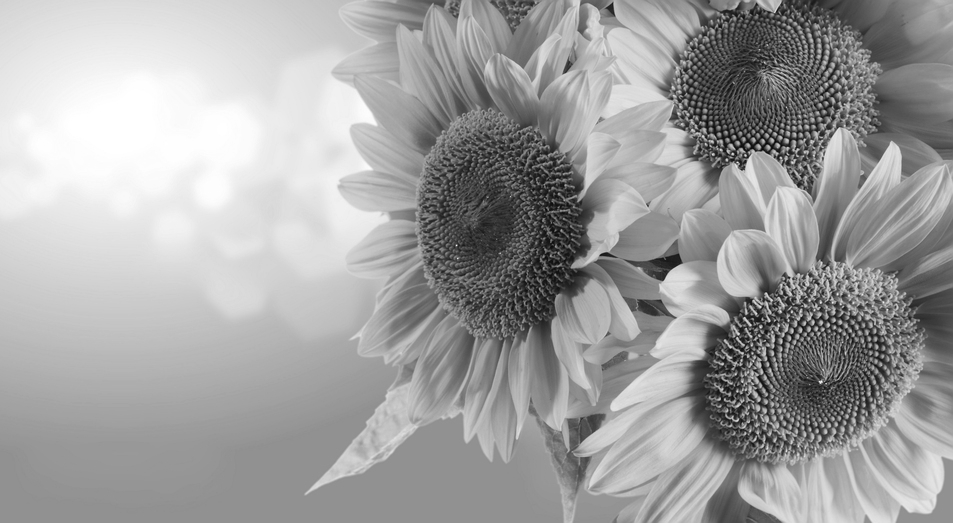
\includegraphics[width=\textwidth]{./media/bn-imagen1.png}
	\caption{Este es el epígrafe de la figura en escala de grises.}
	\end{figure}
	\else
		\ifODT%
		\begin{figure}[!ht]
		\centering
		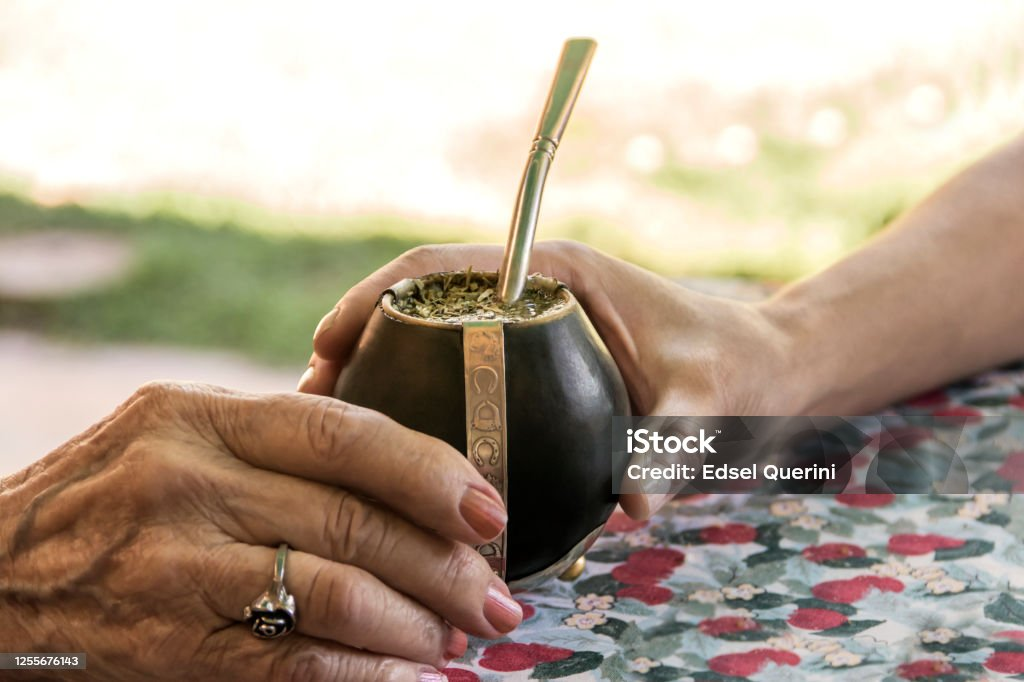
\includegraphics[width=\textwidth]{./media/imagen1.jpg}
		\caption{Este es el epígrafe de la figura a color.}
		\end{figure}
		\else
			\ifEPUB
			\begin{figure}[!ht]
			\centering
			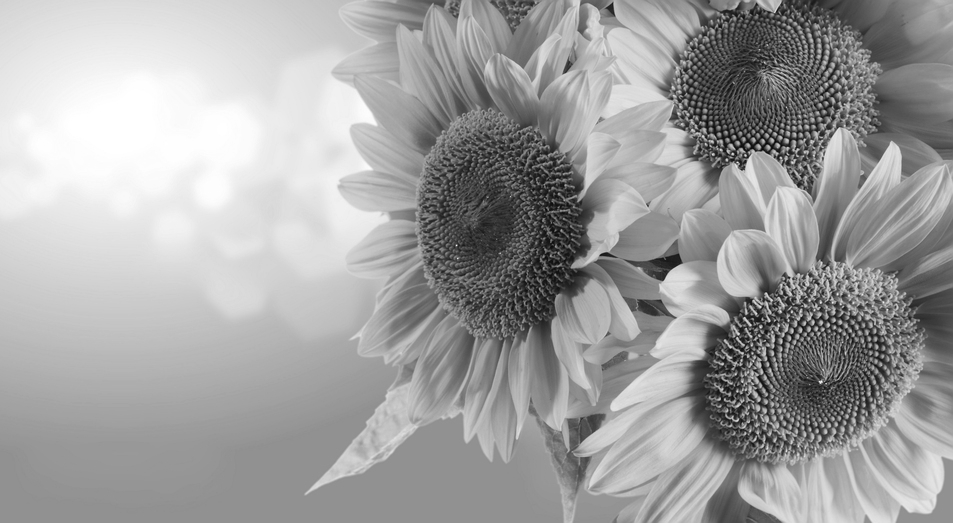
\includegraphics[width=\textwidth]{./media/bn-imagen1.png}
			\caption{Este es el epígrafe de la figura a color.}
			\end{figure}
			\fi
		\fi
	\fi
\fi

\section{SecciónBB}

Esta obra colectiva da continuidad a uno de los programas centrales impulsados por el \gls{@glo201-ceheal} desde su creación en 2019: el estudio de las ideas y del pensamiento económico en su vínculo con la implementación de políticas económicas.\footnote{Nota a pie en una sección del segundo capítulo.}

\backmatter

%Condicional para llevar todas las notas a pie al final del libro como un capítulo.
%Conditional to move all the footnotes to the end of the book as a chapter
\ifEPUB
\begingroup
\parindent 0pt
\parskip 2ex
\def\enotesize{\normalsize}
\theendnotes
\endgroup
\fi

\ifPDF
\printnoidxglossary[type=\acronymtype,title={Índice de siglas}]
\printnoidxglossary[title={Glosario de términos}]
\printbibliography[heading=none,heading=bibintoc]
\else
	\ifBNPDF
	\printnoidxglossary[type=\acronymtype,title={Índice de siglas}]
	\printnoidxglossary[title={Glosario de términos}]
	\printbibliography[heading=none,heading=bibintoc]
	\else
		\ifODT
		\printnoidxglossary[type=\acronymtype,title={Índice de siglas}]
		\printnoidxglossary[title={Glosario de términos}]
		\printbibliography[heading=none,heading=bibintoc]
		\else
			\ifEPUB
			\printnoidxglossary[type=\acronymtype,title={Índice de siglas}]
			\printnoidxglossary[title={Glosario de términos}]
			\chapter{Bibliografía}
			\printbibliography[heading=none]
			\fi
		\fi
	\fi
\fi





\ifPDF
\printindex[names]
\printindex[concepto]
\printindex[onomastico]
\Author{Índice de autoras y autores}
\else
	\ifBNPDF
	\printindex[names]
	\printindex[concepto]
	\printindex[onomastico]
	\Author{Índice de autoras y autores}
% \else
% 	\ifEPUB
% 	\printindex[names]
% 	\printindex[concepto]
% 	\printindex[onomastico]
% 	\fi
	\fi
\fi

\chapter{Colofón}

La composición tipográfica de este libro se realizó utilizando el lenguaje \gls{@glo200-latex} y el software gbTeXpublisher.

Las familias tipográficas utilizadas dentro del libro son: IBM Plex, una superfamilia de tipografía abierta, diseñada y desarrollada conceptualmente por Mike Abbink en IBM con colaboración de Bold Monday y Libertinus, bifurcación de la fuente Linux Libertine, diseñada para el texto del cuerpo y la lectura extendida.

\ifPDF
\newpage
\thispagestyle{empty}
{\textcolor{white}{.}}
\else
	\ifBNPDF
	\newpage
	\thispagestyle{empty}
	{\textcolor{white}{.}}
	\fi
\fi

\end{document}



